\documentclass[3p,times,number]{elsarticle}
\usepackage[utf8]{inputenc}
\usepackage{amsmath,amssymb}
\usepackage{booktabs}
\usepackage{caption}
\usepackage{subcaption}
\usepackage{hyperref}
\usepackage{orcidlink}
\usepackage{graphicx}
\graphicspath{{../img/}}
\captionsetup{font=small,labelfont=bf}
\hypersetup{colorlinks=true,linkcolor=blue,citecolor=blue,urlcolor=blue}

\begin{document}

\begin{frontmatter}

\title{Improving the SegFormer Decoder for Semantic Segmentation by Adding a Depthwise Convolution Block}

\author[spbstu]{Salimli~Ayzek~Muxtar~oglu\corref{cor1}\fnref{msc}~%
\orcidlink{0009-0005-9984-0740}}
\ead{thisisnauchno@gmail.com}
\fntext[msc]{M.Sc.\ student.}

\address[spbstu]{Peter the Great St.~Petersburg Polytechnic University, 29 Politekhnicheskaya St., St.~Petersburg 195251, Russia}

\begin{abstract}
Efficient semantic segmentation networks are usually improved by modifying the token mixer
of the encoder. In a controlled study on Oxford-IIIT Pet, four token mixers are substituted
into an identical SegFormer-B0 architecture under a single training protocol. Mixers that
inherit pretrained attention weights reach the same accuracy (border-class IoU within
$0.0003$) while differing in throughput by a factor of six; the token mixer therefore
determines the cost of the model but not its accuracy. A per-class error analysis locates
the accuracy bottleneck in the decoder. The all-MLP decoder of SegFormer consists of
$1 \times 1$ convolutions only, so its receptive field on the fused feature map equals one
position. Inserting a single depthwise $3 \times 3$ convolution after the fusion step adds
$2816$ parameters ($0.08$\% of the model) without measurable latency and raises mIoU from
$0.8095$ to $0.8161$, border IoU from $0.6004$ to $0.6137$ and mask $\mathrm{mAP}_{50:95}$
from $0.8198$ to $0.8270$. A paired ablation isolates the effect of this convolution. The
modified model is also compared with DeepLabV3+ and YOLOv8s-seg under a shared binary
foreground protocol.
\end{abstract}

\begin{keyword}
semantic segmentation \sep vision transformer \sep SegFormer \sep decoder design \sep
receptive field \sep depthwise convolution
\end{keyword}

\end{frontmatter}

\section{Introduction}

Semantic segmentation assigns a class label $\hat{y}_{ij} = \arg\max_c z_{cij}$ to every
pixel of an image $x \in \mathbb{R}^{3 \times H \times W}$, where
$z \in \mathbb{R}^{C \times H \times W}$ are the predicted logits. The output has the
spatial extent of the input, so a segmentation model must combine global semantic context
with precise localisation.

SegFormer \cite{segformer} combines a hierarchical transformer encoder with a minimal
all-MLP decoder and provides a strong accuracy--efficiency trade-off. Subsequent work has
mainly replaced the encoder token mixer with state space scans \cite{mamba2}, linear
attention \cite{flatten} or convolutional attention \cite{segnext}, which assumes that the
token mixer determines segmentation accuracy. The present work tests this assumption under
controlled conditions and, on the basis of the result, examines the decoder instead.

The contributions are as follows:
\begin{enumerate}
\item a controlled comparison showing that the choice of token mixer does not affect
accuracy when pretrained weights are inherited;
\item a receptive-field analysis identifying the all-MLP decoder as the accuracy bottleneck;
\item a decoder modification with one depthwise $3 \times 3$ convolution (hereafter
SegFormer-B0-DW) that improves all quality metrics at a cost of $2816$ parameters.
\end{enumerate}

\section{Background}

\textbf{SegFormer encoder.} The MiT encoder \cite{segformer,pvt,pvtv2} processes
overlapping patches in four stages with strides $4, 8, 16, 32$ and, for the B0
configuration, channel widths $32, 64, 160, 256$. Self-attention over $N$ tokens costs
$O(N^2 d)$. SegFormer reduces keys and values spatially by a ratio $R$,
$$
X' = \mathrm{SR}(X, R) \in \mathbb{R}^{(N / R^2) \times d},
\qquad K = X' W_K, \quad V = X' W_V,
$$
which lowers the cost to $O(N^2 d / R^2)$ with $R = 8, 4, 2, 1$ across the stages.

\textbf{All-MLP decoder.} Let $F^{(k)} \in \mathbb{R}^{C_k \times H_k \times W_k}$ be the
output of stage $k$. The decoder projects each stage to a common width $D$, resizes it to
stride four and fuses the result:
$$
U^{(k)} = \mathrm{Resize}\!\left(W^{(k)}_{p} \ast_{1 \times 1} F^{(k)}\right),
\qquad
G = W_{f} \ast_{1 \times 1}
\left[\, U^{(1)} \,\|\, U^{(2)} \,\|\, U^{(3)} \,\|\, U^{(4)} \,\right].
$$
Batch normalisation, ReLU, a $1 \times 1$ classifier and bilinear upsampling by four
follow. All convolutions in this path have $1 \times 1$ kernels.

\textbf{Reference models.} DeepLabV3+ \cite{deeplabv3plus} uses a ResNet-50 backbone
\cite{resnet} with atrous spatial pyramid pooling, in which a $3 \times 3$ kernel with
dilation $r$ covers $2r+1$ positions. YOLOv8-seg \cite{yolov8} is an instance segmentation
model that predicts masks $m_n = \sigma(\sum_k \alpha_{n,k} P_k) \odot \mathbb{1}[b_n]$
from shared prototypes $P_k$ cropped by a bounding box $b_n$. The instance formulation
cannot represent classes without object instances, such as the boundary ring used in this
work; the comparison with YOLOv8s-seg is therefore performed on a binary foreground task.

\section{Methods}

\textbf{Dataset and protocol.} Experiments use Oxford-IIIT Pet \cite{pets} with three
classes: background, pet and border (the ambiguity ring around each animal). The official
split is used: $3680$ trainval images ($10$\% held out for monitoring) and $3669$ test
images, resized to $256 \times 256$. All models are trained with AdamW \cite{adamw},
learning rate $3 \times 10^{-4}$ (multiplied by $0.1$ for pretrained encoder parameters),
weight decay $0.01$, polynomial decay with $5$\% warmup, gradient clipping at $1.0$, batch
size $16$, $20$ epochs, flip, scaled crop and brightness augmentation, pixel-wise cross
entropy loss and a fixed seed $1337$.

\textbf{Metrics.} With per-class pixel counts $\mathrm{TP}_c$, $\mathrm{FP}_c$,
$\mathrm{FN}_c$ accumulated over the test set,
$$
\mathrm{IoU}_c = \frac{\mathrm{TP}_c}{\mathrm{TP}_c + \mathrm{FP}_c + \mathrm{FN}_c},
\quad
\mathrm{Dice}_c = \frac{2\,\mathrm{TP}_c}{2\,\mathrm{TP}_c + \mathrm{FP}_c + \mathrm{FN}_c},
\quad
F_{\beta,c} = \frac{(1 + \beta^{2})\, P_c R_c}{\beta^{2} P_c + R_c},
$$
where $P_c$ and $R_c$ are precision and recall; $\beta = 2$ is reported. Mask
$\mathrm{mAP}_{50:95}$ is computed over connected foreground components as the mean of
$101$-point interpolated AP at IoU thresholds $0.50, 0.55, \dots, 0.95$. Latency is the
mean of $25$ forward passes at batch size one after $8$ warmup passes.

\section{Effect of the Token Mixer}

The original efficient self-attention \cite{segformer} is compared with four token mixers
substituted into an identical architecture: reduced-key linear attention \cite{flatten},
fixed-budget gated attention with keys and values pooled to an $8 \times 8$ grid,
convolutional attention \cite{segnext} and a selective state space scan \cite{mamba2}. Table~\ref{tab:mixers} shows that mixers
inheriting the pretrained projection weights reach border IoU between $0.6004$ and
$0.6006$. Mixers with a different parameterisation start from random initialisation and
lose accuracy. Training the same architecture with and without inherited weights gives a
difference of $+0.1018$ mIoU for linear attention and $+0.0430$ for fixed-budget
attention, which exceeds the spread between any two mixers. The token mixer thus determines
inference cost but not accuracy.

\begin{table}[t]
\centering
\small
\caption{Token mixers in an identical architecture under one training protocol.}
\label{tab:mixers}
\begin{tabular}{lccccc}
\toprule
\textbf{Token mixer} & \textbf{Inherits} & \textbf{mIoU} & \textbf{Border IoU} &
\textbf{mAP$_{50:95}$} & \textbf{FPS} \\
\midrule
Efficient self-attention        & yes & 0.8095 & 0.6004 & 0.8198 & 156.9 \\
Reduced-key linear attention    & yes & 0.8093 & 0.6006 & 0.8190 & 136.1 \\
Fixed-budget gated attention    & yes & 0.8092 & 0.6005 & 0.8186 & 143.9 \\
\midrule
Convolutional attention         & no  & 0.7871 & 0.5651 & 0.7826 & 141.2 \\
Selective state space scan      & no  & 0.7549 & 0.5202 & 0.7345 & 24.0 \\
\bottomrule
\end{tabular}
\end{table}

\section{Proposed Decoder Modification}

\subsection{Error analysis}

The per-class IoU of the baseline is $0.9412$ for background, $0.8869$ for pet and
$0.6004$ for border. Two explanations of the border deficit are excluded.
\emph{Decoder resolution:} passing the ground truth through the same stride-four bottleneck
(one-hot encoding, bilinear downsampling and upsampling, arg max) gives an upper bound of
$0.9101$ border IoU, far above the model value. \emph{Calibration:} scaling the border
logit by $2.5$ raises border IoU by $0.0095$ but lowers mIoU from $0.7989$ to $0.7956$;
the mean predicted border probability on border pixels is already $0.6496$. The error is
therefore caused by inaccurate localisation of the ring rather than by resolution or
calibration.

\subsection{Receptive field of the decoder}

Let $G \in \mathbb{R}^{D \times H/4 \times W/4}$ be the fused feature map and $\rho$ the
receptive field of the decoder on $G$. Since all operations after fusion are $1 \times 1$
convolutions, normalisation or pointwise nonlinearities,
$$
z_{:,i,j} = g\!\left( G_{:,i,j} \right), \qquad \rho = 1,
$$
and each stride-four cell is classified independently of its neighbours. Determining
whether a cell lies on the boundary requires information about adjacent cells. A depthwise
$3 \times 3$ convolution \cite{mobilenet} inserted after fusion gives
$$
z_{:,i,j} = g\!\left( \sum_{|a| \le 1} \sum_{|b| \le 1}
w_{a,b} \odot G_{:,\, i+a,\, j+b} \right), \qquad \rho = 3,
$$
which corresponds to $12$ pixels at input resolution. The block contains
$D \times 3 \times 3 = 2304$ weights and $512$ normalisation parameters, $2816$ in total,
against $3\,714\,915$ parameters of the baseline. The resulting architecture is shown in
Fig.~\ref{fig:arch}.

\begin{figure}[t]
\centering
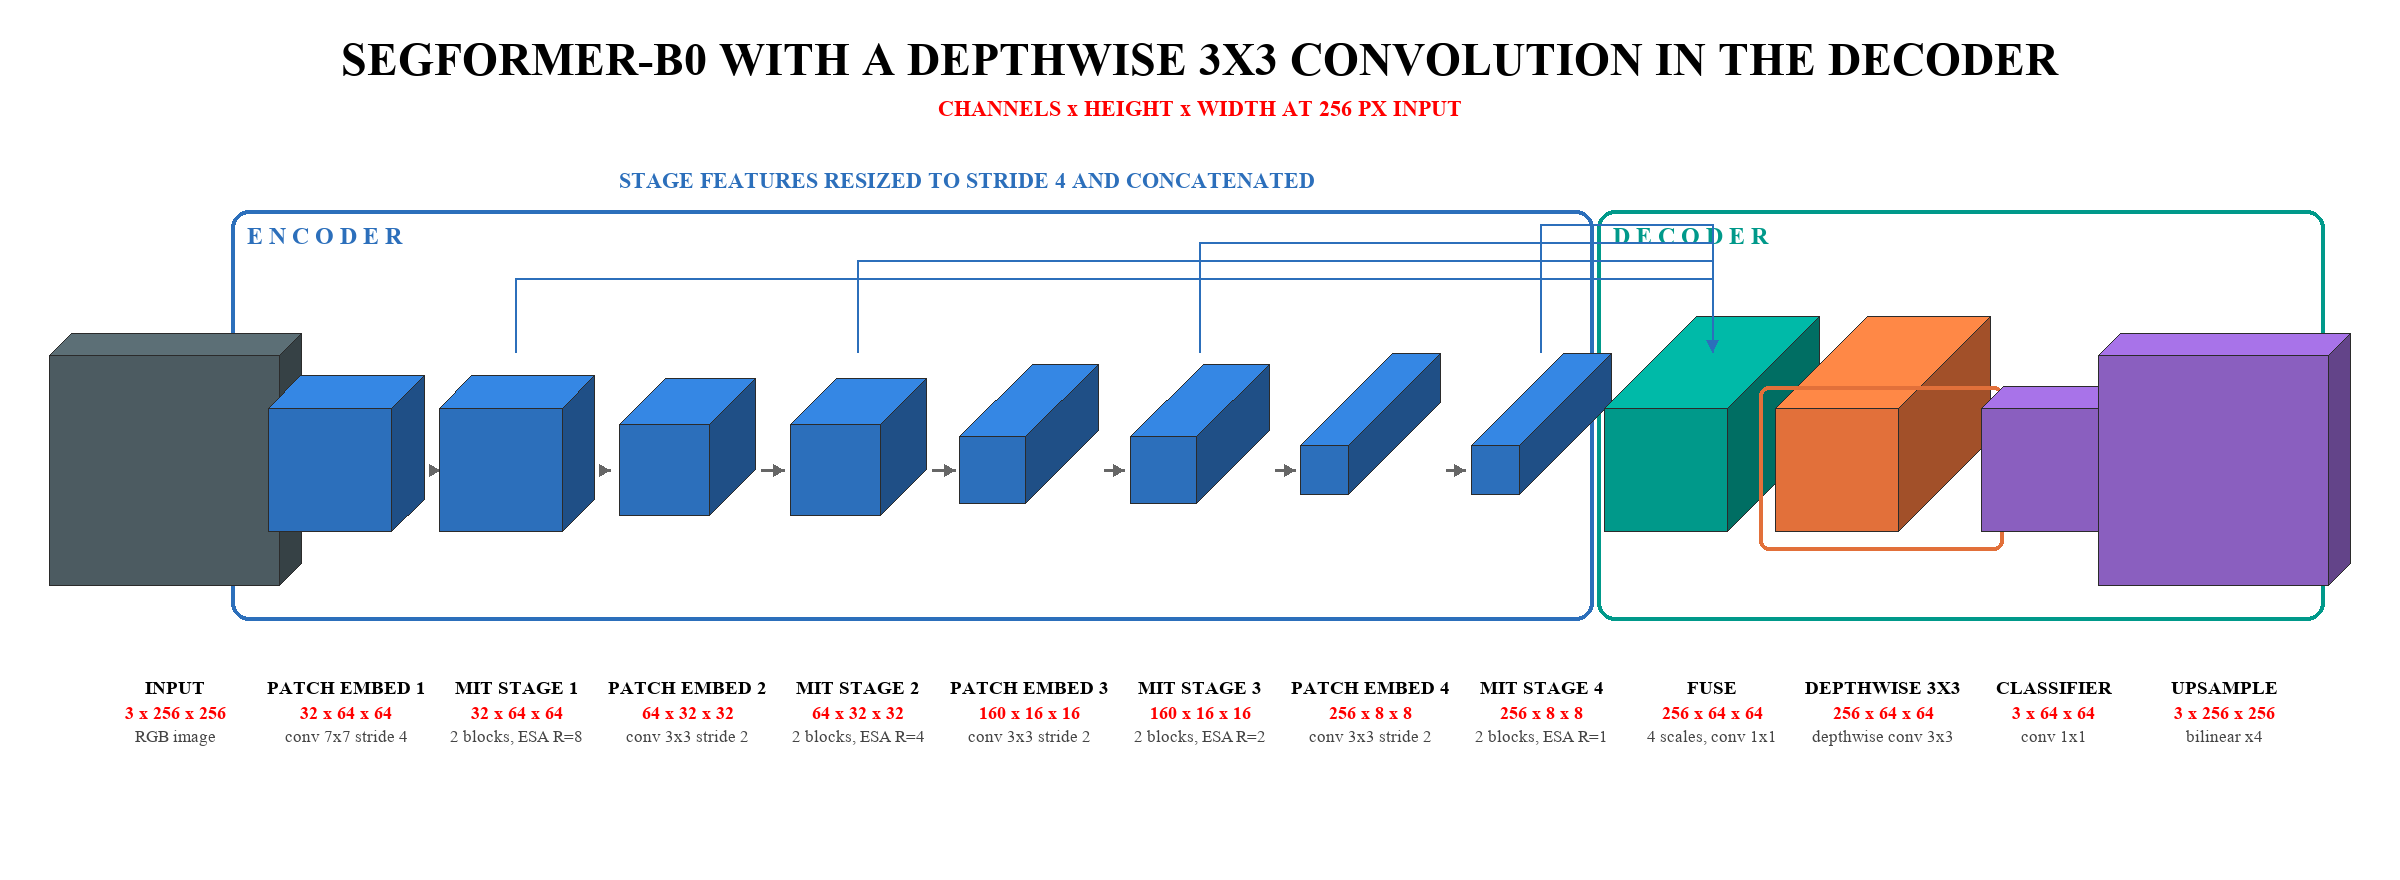
\includegraphics[width=\textwidth]{architecture.png}
\caption{SegFormer-B0-DW. The MiT-B0 encoder and the all-MLP fusion are unchanged; a
depthwise $3 \times 3$ convolution is inserted between the fusion and the classifier.}
\label{fig:arch}
\end{figure}

\section{Results}

\subsection{Paired ablation}

Two models differing only by the depthwise convolution are trained with identical widths,
protocol and seed (Table~\ref{tab:ablation}). The largest gain is observed for the border
class ($+0.0121$ IoU), while background and pet improve by $0.0021$ and $0.0046$, in
agreement with the receptive-field analysis: region interiors are classified correctly from
a single feature vector, whereas boundaries require neighbouring context.

\begin{table}[t]
\centering
\small
\caption{Paired ablation: the two decoders differ by one depthwise $3 \times 3$
convolution.}
\label{tab:ablation}
\begin{tabular}{lccccc}
\toprule
\textbf{Decoder} & \textbf{Params} & \textbf{mIoU} & \textbf{Border IoU} &
\textbf{mAP$_{50:95}$} & \textbf{FPS} \\
\midrule
$1 \times 1$ only, $\rho = 1$           & 3\,714\,915 & 0.8102 & 0.6016 & 0.8205 & 163.8 \\
with depthwise $3 \times 3$, $\rho = 3$ & 3\,717\,731 & \textbf{0.8161} & \textbf{0.6137} &
\textbf{0.8270} & 161.9 \\
\midrule
Difference & $+2816$ & $+0.0059$ & $+0.0121$ & $+0.0065$ & $-1.9$ \\
\bottomrule
\end{tabular}
\end{table}

\subsection{Comparison with the baseline and reference models}

DeepLabV3+ and YOLOv8s-seg have no border class, so all models are additionally evaluated
on a binary foreground task in which pet and border are merged; VOC and COCO cat and dog
classes are mapped to foreground for the reference models. Binary scores of the SegFormer
models are derived from their three-class confusion matrices (deviation from a direct
measurement below $0.0003$). Table~\ref{tab:main} and Fig.~\ref{fig:results} summarise the
results.

\begin{table*}[t]
\centering
\small
\caption{Comparison on the Oxford-IIIT Pet test split ($3669$ images). FG denotes the
binary foreground task.}
\label{tab:main}
\begin{tabular}{lcccccccc}
\toprule
\textbf{Model} & \textbf{Params} & \textbf{FG IoU} & \textbf{FG Dice} & \textbf{FG F2} &
\textbf{mAP$_{50:95}$} & \textbf{mIoU} & \textbf{Border IoU} & \textbf{FPS} \\
\midrule
SegFormer-B0-DW   & 3.72 M  & \textbf{0.9227} & \textbf{0.9598} & \textbf{0.9569} &
\textbf{0.8270} & \textbf{0.8161} & \textbf{0.6137} & \textbf{161.9} \\
SegFormer-B0-BR   & 3.50 M  & 0.9225 & 0.9597 & 0.9560 & 0.8271 & 0.8162 & 0.6138 & 116.0 \\
SegFormer-B0      & 3.71 M  & 0.9199 & 0.9583 & 0.9558 & 0.8198 & 0.8095 & 0.6004 & 156.9 \\
YOLOv8s-seg       & 11.82 M & 0.8397 & 0.9129 & 0.8801 & 0.6196 & --- & --- & 152.2 \\
DeepLabV3+-R50    & 42.00 M & 0.8329 & 0.9088 & 0.8724 & 0.6398 & --- & --- & 27.4 \\
\bottomrule
\end{tabular}
\end{table*}

\begin{figure*}[t]
\centering
\begin{subfigure}{0.49\textwidth}
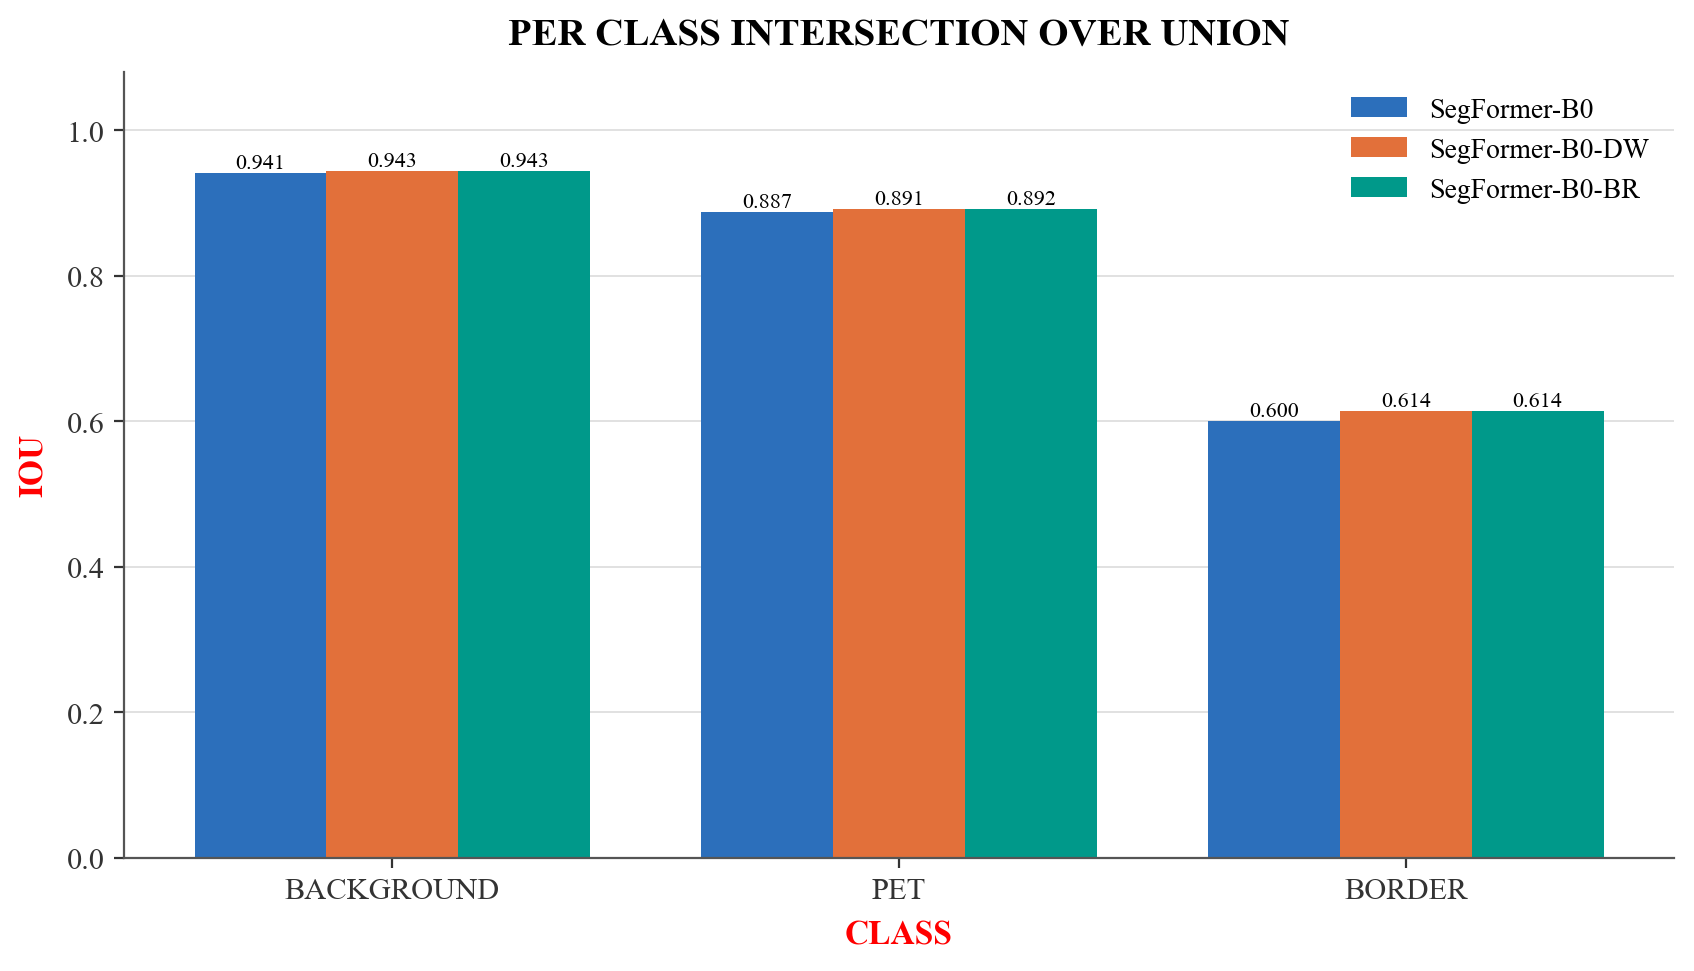
\includegraphics[width=\textwidth]{perclass.png}
\caption{Per-class IoU.}
\label{fig:perclass}
\end{subfigure}
\hfill
\begin{subfigure}{0.49\textwidth}
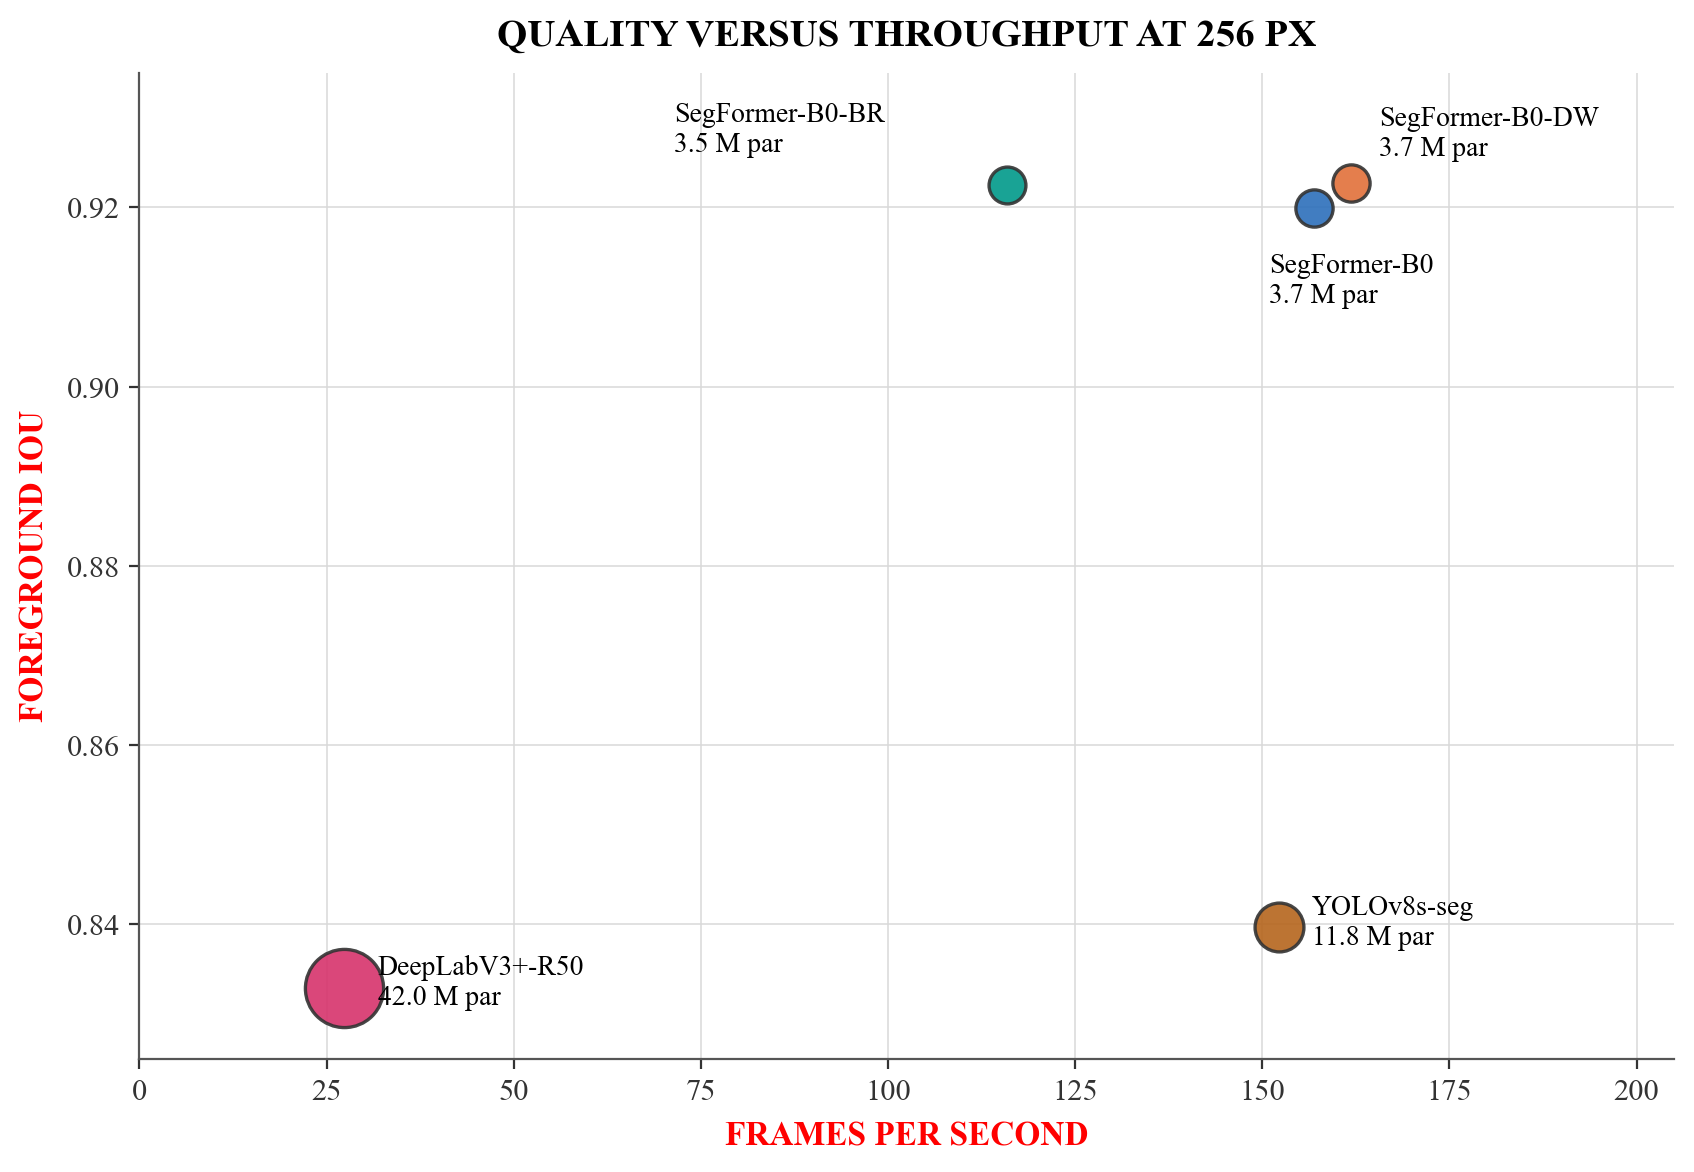
\includegraphics[width=\textwidth]{pareto.png}
\caption{Foreground IoU against throughput.}
\label{fig:pareto}
\end{subfigure}
\caption{Per-class quality and the quality--throughput trade-off of the compared models.}
\label{fig:results}
\end{figure*}

\begin{figure}[t]
\centering
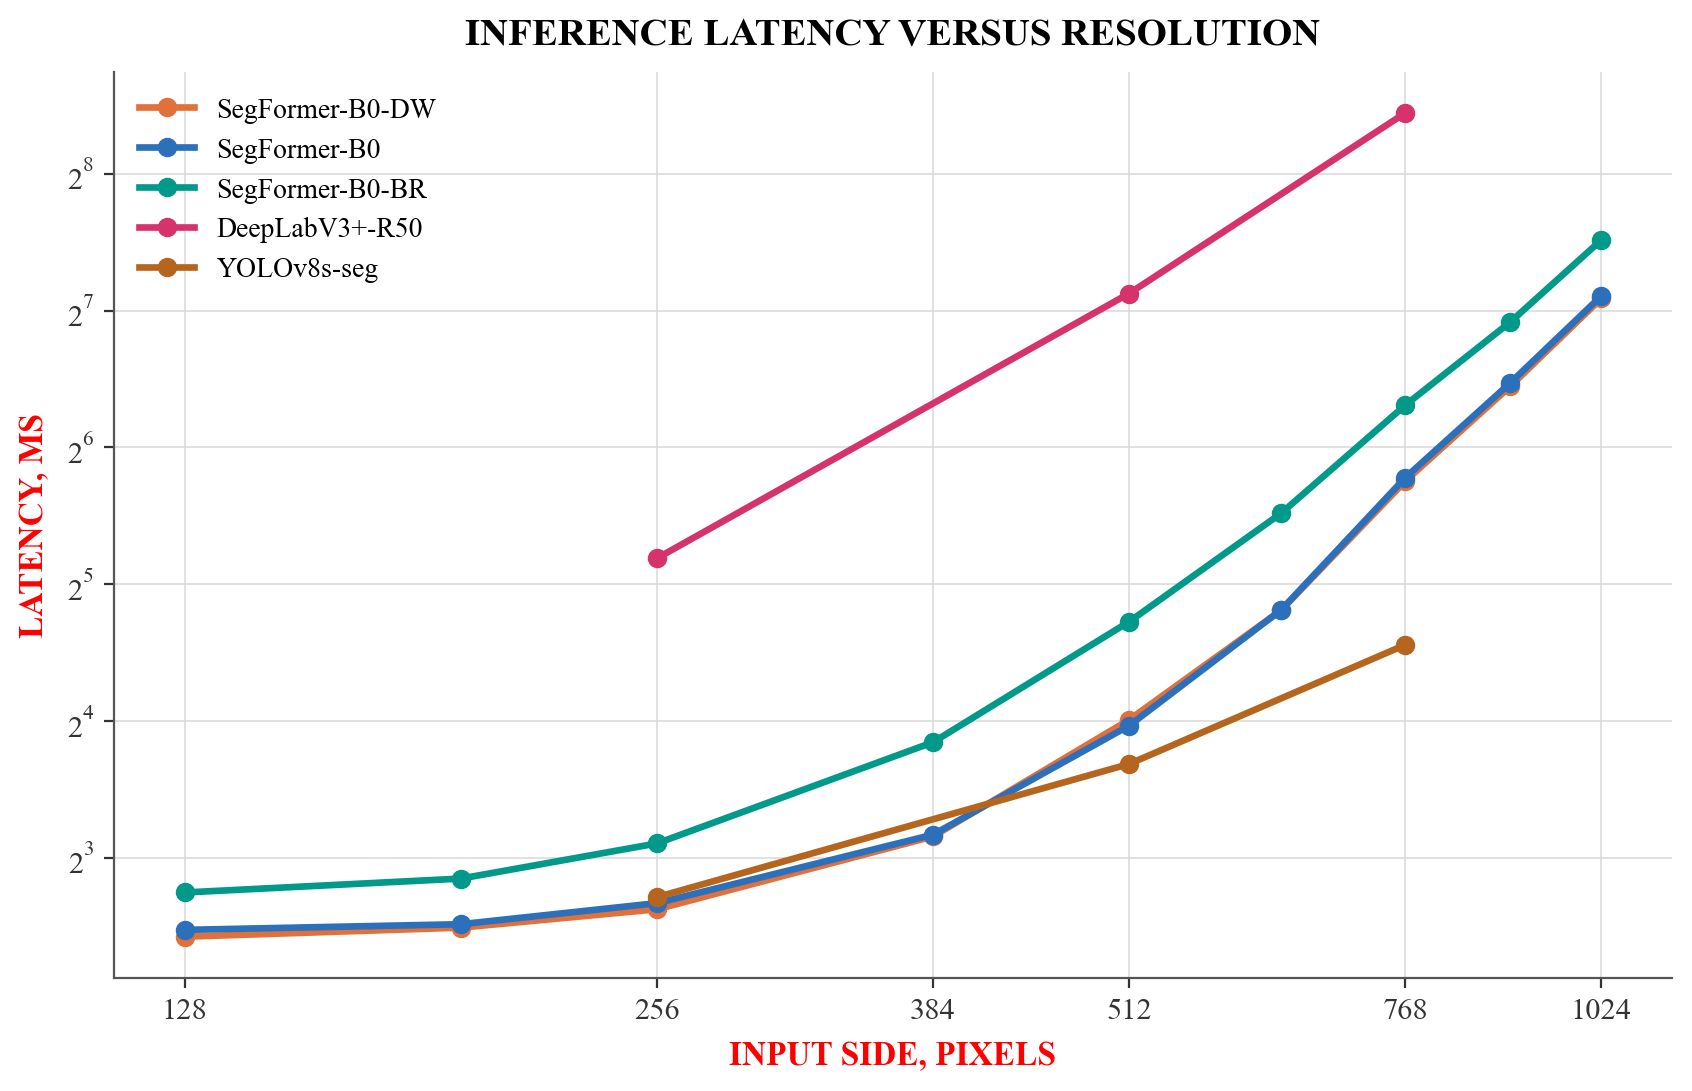
\includegraphics[width=0.6\textwidth]{latency.png}
\caption{Inference latency against input resolution.}
\label{fig:latency}
\end{figure}

SegFormer-B0-DW exceeds the baseline in all quality metrics; its latency coincides with that
of the baseline within measurement noise at all resolutions (Fig.~\ref{fig:latency}).
The reference models were evaluated as published checkpoints without fine-tuning on this
dataset, so the gap of about $0.08$ in foreground IoU reflects in-domain training rather
than architectural inferiority. DeepLabV3+ requires $11$ times more parameters and is six
times slower than SegFormer-B0-DW. YOLOv8s-seg has the lowest mask AP ($0.6196$) because a
missed detection removes the entire object from the prediction.

\section{Discussion}

\textbf{Mechanism.} SegFormer-B0-BR in Table~\ref{tab:main} denotes an alternative decoder
with a full-resolution detail branch and a supervised boundary gate,
$z = z_{\text{sem}} + \sigma(b) \odot \Delta(\text{detail}, \text{semantic})$. Removing
the boundary gate and its supervision leaves mIoU unchanged ($0.8167$ against $0.8162$), as
does removing the detail branch ($0.8163$). Both variants retain a depthwise convolution in
the fusion path, which the paired ablation identifies as the source of the gain. The
improvement is therefore explained by the enlarged receptive field of the decoder rather
than by the additional branches, which reduce throughput from $161.9$ to $116.0$ FPS.

\textbf{Limitations.} The evaluation uses one dataset with three classes and one salient
object per image; the results may not transfer to ADE20K or Cityscapes. The baseline is a
fine-tuned SegFormer-B0 rather than a state-of-the-art model. All timings were obtained on
Apple Silicon with the Metal backend and may differ on other hardware. The reference models
were not fine-tuned on the dataset.

\section{Conclusion}

Under a fixed training protocol, token mixers that inherit pretrained weights yield the same
segmentation accuracy while differing by a factor of six in throughput. The accuracy
bottleneck of SegFormer lies in its all-MLP decoder, whose receptive field on the fused
feature map equals one position. Adding a single depthwise $3 \times 3$ convolution after
the fusion step increases the receptive field to three positions and raises mIoU from
$0.8095$ to $0.8161$, border IoU from $0.6004$ to $0.6137$ and mask
$\mathrm{mAP}_{50:95}$ from $0.8198$ to $0.8270$ at a cost of $2816$ parameters and no
measurable latency.

\begin{thebibliography}{99}

\bibitem{segformer}
E. Xie, W. Wang, Z. Yu, A. Anandkumar, J. Alvarez, P. Luo.
SegFormer: Simple and Efficient Design for Semantic Segmentation with Transformers.
\textit{NeurIPS}, 2021.

\bibitem{mamba2}
T. Dao, A. Gu.
Transformers are SSMs: Generalized Models and Efficient Algorithms Through Structured State
Space Duality.
\textit{ICML}, 2024.

\bibitem{flatten}
D. Han, X. Pan, Y. Han, S. Song, G. Huang.
FLatten Transformer: Vision Transformer using Focused Linear Attention.
\textit{ICCV}, 2023.

\bibitem{segnext}
M.-H. Guo, C.-Z. Lu, Q. Hou, Z. Liu, M.-M. Cheng, S.-M. Hu.
SegNeXt: Rethinking Convolutional Attention Design for Semantic Segmentation.
\textit{NeurIPS}, 2022.

\bibitem{pvt}
W. Wang, E. Xie, X. Li, D. Fan, K. Song, D. Liang, T. Lu, P. Luo, L. Shao.
Pyramid Vision Transformer: A Versatile Backbone for Dense Prediction without Convolutions.
\textit{ICCV}, 2021.

\bibitem{pvtv2}
W. Wang, E. Xie, X. Li, D. Fan, K. Song, D. Liang, T. Lu, P. Luo, L. Shao.
PVTv2: Improved Baselines with Pyramid Vision Transformer.
\textit{Computational Visual Media}, 2022.

\bibitem{deeplabv3plus}
L.-C. Chen, Y. Zhu, G. Papandreou, F. Schroff, H. Adam.
Encoder-Decoder with Atrous Separable Convolution for Semantic Image Segmentation.
\textit{ECCV}, 2018.

\bibitem{resnet}
K. He, X. Zhang, S. Ren, J. Sun.
Deep Residual Learning for Image Recognition.
\textit{CVPR}, 2016.

\bibitem{yolov8}
G. Jocher, A. Chaurasia, J. Qiu.
Ultralytics YOLOv8. 2023.

\bibitem{pets}
O. M. Parkhi, A. Vedaldi, A. Zisserman, C. V. Jawahar.
Cats and Dogs.
\textit{CVPR}, 2012.

\bibitem{adamw}
I. Loshchilov, F. Hutter.
Decoupled Weight Decay Regularization.
\textit{ICLR}, 2019.

\bibitem{mobilenet}
A. G. Howard, M. Zhu, B. Chen, D. Kalenichenko, W. Wang, T. Weyand, M. Andreetto, H. Adam.
MobileNets: Efficient Convolutional Neural Networks for Mobile Vision Applications.
\textit{arXiv:1704.04861}, 2017.

\end{thebibliography}

\end{document}